\chapter{Parallelizing Sparse LU Decomposition}
\label{chapter:parLU}

\section{Level of Granularity}

One of the most important steps in designing a parallel algorithm is to determine the 
level of granularity of the operations to be scheduled.
The LU decomposition of a sparse matrix naturally has a
fine-grain parallelism between individual arithmetic operations because of large 
number of zero elements. This granularity can be exploited effectively using a set 
using a set of small processing elements operating in parallel. Since the operations 
to be scheduled are large in number, the latency of the storage unit and throughput of PEs
become the major contributing factors towards the performance of the entire system.
\\
A medium grain parallelism can also be defined over the LU factorization process by dividing 
arithmetic operations into the sets of operations required to compute one column. 
Gilbert-Peierls algorithm provides the information about the 
columns required in computation of certain column. So we can process 
multiple columns in parallel. 
A directed acyclic graph (DAG) can be used to define dependency among the 
columns i.e. each node in the DAG represents a column and its parents represent the column required to 
compute the given column. The scheduler can schedule the column computation operations according to the graph. 
Such kind of parallelism is easy to extract using the Gilbert-Peierls algorithm [\ref{algo:GP}]. 
The degree of parallelism increases with the number of columns in the matrix as more and more independent 
sets of columns can be found. However, this may cause load imbalance in cases where only 
a few floating point operations are required for an entire column operation.
\\
We can also extract coarse-grained parallelism by dividing the columns
into disjoint sets of dependent column and each set
can be computed independently. This project utilizes the first approach of 
extracting fine-grain parallelism by scheduling individual MAC and divide operations. 
this kind of approach is ideal for network like systems where each node has enough computational
resources to compute set of dependent columns.
\\
Our implantation is geared towards extracting fine grain parallelism. Modern 
FPGAs can support a considerable number of pipelined MAC and divide units along with the 
low latency on-chip BRAMs of quick data access. So naturally, FPGAs are well 
equipped for handling large number of basic tasks. The latency of arithmetic operations
depends on the pipeline depth of processing elements and hence is fixed and known to the scheduler.
The scheduler can leverage this knowledge to optimize memory operations.

\section{The Hardware Architecture}
The hardware should consists of a set of basic arithmetic processing units which can 
access local low latency memory in parallel to fully utilize the capabilities of 
an FPGA. At the same time it should be easily scalable according th requirements
and available resources with. The on chip BRAMs have limited memory and may not
be sufficient hence the hardware should have access to the external memory.
Figure \ref{fig:ParLU:hwArch} shows the overview of proposed architecture. The 
switch network provides simple and easy access to all the BRAM ports and PE ports
allowing to send operands from one source to multiple destinations simultaneously.
Also it is easy to add new BRAMs and PEs to the system by extending the number of connections
of the switch bar. The entire system can be controlled with very basic information such as 
switch box connection an operations to be performed at each BRAM and PE port and hence.
The design philosophy is similar to the  Very Long Instruction World (VLIW) processor
architecture.
\begin{figure}
    \centering
    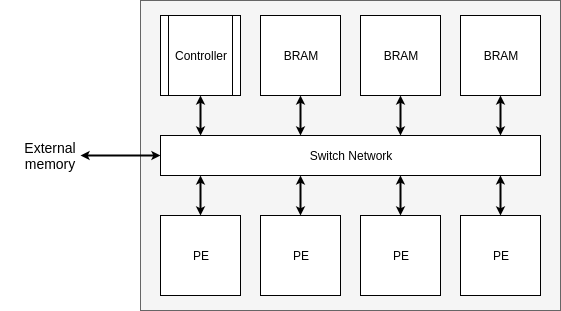
\includegraphics[width = 0.75\linewidth]{./ParallelLU/hardwareOverView.png}
    \caption{Overview of the proposed hardware architecture}
    \label{fig:ParLU:hwArch}
\end{figure}


\section{Pivoting}
Numerical stability is also an important factor in solving linear systems. 
Pivoting method is used to handle the numerical instability that may arise because
of numerical cancellation of diagonal element. There is a trade off between the stability
and sparsity requirements for pivot selection are often contradictory as pivot 
selection changes the matrix structure and may increase number of fill-ins. Since our
method expects that the matrix structure is remains the same, we can not implements the 
actual pivoting step in our design. This problem can be solved easily by 
replacing any tiny pivots with $\sqrt{\epsilon}\Vert A \Vert$ where $\epsilon$ is a machine precision 
and $\Vert A \Vert$ is the norm of the matrix $A$. (refer \cite{Nechma})